\documentclass[11pt,a4paper]{article}
\usepackage[margin=24mm]{geometry}
\usepackage{fontspec}
\setmainfont[Path=../qmsve/fonts/]{ipaexg.ttf}
\setmonofont[Path=../qmsve/fonts/]{DejaVuSansMono.ttf}
\XeTeXlinebreaklocale "ja"
\XeTeXlinebreakskip=0pt plus 1pt
\usepackage{amsmath,amssymb,amsthm,mathtools,booktabs,graphicx,hyperref}
\hypersetup{hidelinks}
\emergencystretch=3em
\newtheorem{theorem}{定理}
\newtheorem{proposition}[theorem]{命題}
\newtheorem{corollary}[theorem]{系}
\newcommand{\R}{\mathbb R}
\newcommand{\ket}[1]{\lvert #1\rangle}
\newcommand{\cP}{\mathcal P}
\title{事前情報に頑健なQSVTフィルタ選択：\\ギャップなしバイアスと有限予算リスク}
\author{}
\date{}
\begin{document}
\maketitle
\begin{abstract}
スペクトルフィルタでは、条件付きバイアスだけでなく、棄却された準備と有限測定の費用を
数える必要がある。本稿は、最小値を含む区間と初期目標質量下界だけを入力とする、実QSVT
フィルタと平均推定器の限定モデルを扱う。ギャップpromiseを選択に用いない。
二点バイアス条件、上端零化の損失保証、厳密な最悪受理確率から、証明付き多項式選択を
構成する。さらに成功数固定の停止則と総予算固定を区別し、回路が理想的でも残る有限試行の
条件付き平均二乗誤差・無出力確率を記述する。その最悪条件付きリスクが高々3固有値で
達成されることを証明し、既知の逆二項モーメント上界から、事前中点を含む有限予算選択を
構成する。解析的な事前保証を持つ6個の小規模イジング鎖で、標本誤差、バイアス下限、
無出力と予算依存の選択を検証し、計228万回のサンプリングを実施した。
有限サンプリングやモーメント支持の議論そのものは既知であり、貢献は固定された
フィルタ・推定器でのスペクトルリスク特徴づけと証明付き選択への接続に限定する。
一般的な量子優位や新しいQSVT原理は主張しない。
\end{abstract}

\section{はじめに}
量子特異値変換（QSVT）はブロックエンコードされた行列に多項式応答を実装する
\cite{Gilyen,Martyn}。問題に合う関数を選ぶ柔軟性は、選択に用いる情報が実際に
利用可能であり、準備・正規化・読出し・棄却の費用を算入した場合に意味を持つ。
低次数で条件付き誤差が小さい関数でも、受理確率が小さければ推定器全体は高価になり得る。

本稿は、非適応の実多項式フィルタと正規化右Gram作用素の独立Bernoulli測定という、
検証可能な設定に限定して関数選択を具体化する。最小値を含む区間とその初期質量下界は
与えられるが、ギャップは仮定しない。設計は、その情報と整合するすべての有限
スペクトルで働く必要があり、真の固有値を見てから都合のよい関数を選ばない。
位相推定や現代的な基底energy推定器全般を置き換える方法とは位置づけない。

解析は三段階からなる。一様平均バイアスを二energy間の不等式で特徴づけ、
応答に$1-x$を掛けることで上端零化しても受理確率の損失が制御できることを示す。
上端零化後は、最悪受理確率が目標区間の最小透過率と重なり下界の積に一致するため、
再試行費用を直接制御する半無限線形計画が得られる。
最後に、連続区間の可行性証明と補正付き双対境界を用いて選択の精度を保証する。

\paragraph{既存研究との関係}
cosineべき乗、応答比、shift、振幅増幅による基底状態準備は既存手法である\cite{Ge}。
既知の孤立目標に対する最適多項式projector\cite{LinTong}、cosine・Gaussian
フィルタと仮想的なフィルタ後期待値\cite{Lu,He}も研究されている。
Filtered QPEはフィルタ費用と重なりを明示的に扱い、複数基底と既知中心のminimax構成を
含む\cite{FQPE}。wall-Chebyshev研究は粗いenergy情報への頑健性と受理費用を評価する
\cite{Wall}。最近の制約付きQSP minimax研究も、有限点と連続可行性の差、最適化と
位相合成の接続を扱う\cite{Constrained}。
したがって線形計画、minimax、多項式のBernstein分割、QSP合成自体は背景技術であり
\cite{Charnes,Farouki,DongPhase}、本稿の発明とはしない。

限定した貢献は、上端零化の受理係数、未知最小値の結合制約と正確な再試行解釈、
および特定のgap-free平均推定器に対する証明付き選択である。
既知中心のrejection bandと異なり、事前区間の全目標とそれより大きい全固有値を
結ぶ制約を課す。忠実度保証と異なり、近接した目標外成分が残ることを許す。
これは問題設定の違いを示すもので、既存推定器への優位性や各構成要素の普遍的な
優先性を意味しない。

\section{情報・oracle・推定器モデル}\label{sec:model}
既知の$\alpha\geq\|A\|_2>0$に対し$B=A/\alpha$、$G=B^\dagger B$とし、
スペクトルを$[0,1]$に置く。最小固有値$e=\lambda_{\min}(G)$に関する入力は
\begin{equation}\label{eq:prior}
 0\leq e\leq u<1,\qquad p_0\geq a,\quad 0<a<1
\end{equation}
であり、$p_0$は最小固有空間への初期総質量である。
目標外固有値は$e$へ任意に近づいてよく、縮退は目標質量を合算して扱う。
真のスペクトルや重みを古典的に読めるとは仮定しない。
数値生成器は検証のためにそれらを知るが、フィルタ選択には渡さない。

実振幅$P$は$[0,1]$上$|P|\leq1$、$[0,u]$上非零とする。
多項式では符号を選び目標区間上$P>0$とできる。
受理確率と事後平均は
\[
 Z_P=\sum_i p_iP(\lambda_i)^2,\qquad
 \mu_P=\frac{\sum_i p_iP(\lambda_i)^2\lambda_i}{Z_P}
\]
である。入力条件を満たす全有限スペクトル・重みの集合を$\mathfrak I(a,u)$とし、
\[
S(P)=\inf_{I\in\mathfrak I(a,u)}Z_P(I)
\]
と定める。
全入力で$\mu_P-e\leq b$なら、$P$はバイアス$b$で可行と呼ぶ。
実装時は共通余裕$\kappa=19/20$を多項式全体に一度だけ掛ける。
条件付き平均は変わらず、受理確率が$\kappa^2$倍になる。

$x=\lambda$で次数$n$の$P$は、正規化特異値$s$では$P(s^2)$という偶次数$2n$の
応答である。controlled singular-value signal、その逆、および標準QSVT反射が
利用可能とする。QSPユニタリと逆のcontrolled分枝を直列に実行する保守的な
実数応答の抽出規約では、フィルタ試行一回に$4n$ signal呼出しを数える。
全候補でこの規約を共通化し、物理ゲートやT-countの評価とは区別する。
状態準備の費用を$c_\psi$、直列深さを$d_\psi$とすれば、深さ上限は
$d_\psi+4n+1\leq D$である。最後の1回は読出しである。
数値モデルでは保守的に$d_\psi=c_\psi$と置く。

受理状態上の$B$ block-encodingのsuccess flagは、平均$\mu_P$のBernoulli変数となる。
全正規化Gram誤差$E$をバイアス$0<b<E$と標本誤差$E-b$に分ける。
\begin{equation}\label{eq:shots}
 M(b)=\left\lceil\frac{\log(2/\delta)}{2(E-b)^2}\right\rceil
\end{equation}
個の独立受理コピーで、Hoeffdingから確率$1-\delta$以上で
$|\widehat\mu-e|\leq E$となる。
失敗時は試行全体を捨てて初期状態からやり直し、振幅増幅や途中再利用は行わない。
幾何待ち時間と受理分布の独立性により、最悪期待query費用は正確に
\begin{equation}\label{eq:cost}
 J(P,n,b)=M(b)\left[\frac{c_\psi+4n}{\kappa^2S(P)}+1\right]
\end{equation}
となる。

右空間の最小特異値を$\sigma_R(A)=\min_{\|v\|=1}\|Av\|=\alpha\sqrt e$と定義する。
読出しを$[0,1]$へclipして平方根を取れば、誤差は$\alpha\sqrt E$以下である。
横長行列では右核により零となり、通常のthin SVDの最小値と異なり得る。
事前情報の取得費用は共通の追加入力費であり、ここでは最適化しない。
追加測定で事前区間を狭める適応法も対象外である。

\paragraph{計算しないbaseline}
$u/2$を返せば$e$を$u/2$以内に、$\alpha\sqrt u/2$を返せば$\sigma_R$を
$\alpha\sqrt u/2$以内に推定できる。
要求精度がこれで満たされるなら、それを選ぶべきである。
本実験は$u>4E$とし、特異値誤差$\alpha\sqrt E$で見ても事前中点だけでは解けない。
また非フィルタ平均の最悪バイアスは$1-a$であり、その配分以上を許す場合だけ可行である。
これは特定平均推定器についての事実で、非フィルタ量子アルゴリズム全般の下界ではない。

\section{二点条件と上端零化}
\begin{proposition}[一様平均バイアスの条件]\label{prop:pair}
目標区間で非零の$P$がバイアス$b>0$で可行である必要十分条件は、
全$0\leq e\leq u$、$e+b<x\leq1$について
\begin{equation}\label{eq:pair}
 (1-a)(x-e-b)P(x)^2\leq abP(e)^2
\end{equation}
が成り立つことである。
\end{proposition}
\begin{proof}
必要性は、$e,x$に質量$a,1-a$を置いて正の事後分母を掛ければ得られる。
十分性では実際の目標質量$p_0\geq a$を考える。
$x-e\leq b$の左辺は非正なので、目標外条件付き分布で平均して
\[
 \sum_{i>0}p_i(\lambda_i-e-b)P(\lambda_i)^2
 \leq\frac{(1-p_0)ab}{1-a}P(e)^2\leq p_0bP(e)^2
\]
を得る。これはバイアス条件を分母で払った式に一致する。
\end{proof}
固定$e$、目標質量がちょうど$a$の場合、最大バイアスは同じ平均議論から
\begin{equation}\label{eq:two-point}
 \max_{e\leq x\leq1}
 \frac{(1-a)(x-e)P(x)^2}{aP(e)^2+(1-a)P(x)^2}
\end{equation}
に一致する。最大点に目標外全質量を置く二準位例が達成する。
この線形分数の極値原理自体は古典的である\cite{Charnes}。

\begin{theorem}[制御された上端零化]\label{thm:null}
$u+b<1$とし、連続$P$がバイアス$b$で可行、$|P|\leq1$とする。
$Q(x)=(1-x)P(x)$も可行、$|Q|\leq1$、$Q(1)=0$であり、
\begin{equation}\label{eq:null-factor}
 S(Q)\geq(1-u)(1-u-b)S(P)
\end{equation}
を満たす。$P$の次数が$n$以下なら、$Q$のGram次数は$n+1$以下である。
\end{theorem}
\begin{proof}
$x\geq e$なら$0\leq1-x\leq1-e$なので、式\eqref{eq:pair}に
$(1-e)^2$を掛ければ$Q$の条件を得る。
$m=\min_{[0,u]}P^2>0$、最小点を$e_*$とする。
全入力で$Z_Q\geq a(1-u)^2m$。
一方、$P$には$e_*,1$に質量$a,1-a$を置く許容入力を使え、式\eqref{eq:pair}から
\[
 S(P)\leq am+(1-a)P(1)^2
 \leq am\frac{1-e_*}{1-e_*-b}
 \leq am\frac{1-u}{1-u-b}.
\]
二つの式を組み合わせればよい。
\end{proof}

\begin{corollary}[制約の費用]\label{cor:restriction}
同じ$b,M,\kappa$のもとで、次数$n$の応答を上端零化した次数$n+1$の応答へ変えると、
最悪期待費用の増加率は
\begin{equation}\label{eq:restriction-cost}
 \frac{c_\psi+4(n+1)}{c_\psi+4n}\frac1{(1-u)(1-u-b)}
\end{equation}
以下である。ただし追加次数が深さ上限内に収まる必要がある。
\end{corollary}

\begin{theorem}[上端零化後の正確な受理確率]\label{thm:success}
$P$が連続で、$P(1)=0$、$[0,u]$上$P>0$なら、
$\tau(P)=\min_{[0,u]}P$について
\begin{equation}\label{eq:success}
 S(P)=a\tau(P)^2
\end{equation}
である。
\end{theorem}
\begin{proof}
目標成分が下界を与える。$P$の最小点に質量$a$、$1$に残りの質量を置けば等号となる。
\end{proof}
この受理確率の一致と上端零化の損失係数が、制限したクラスを使う構造的な理由である。
振幅増幅や適応フィルタとの比較ではない。

\section{多項式の選択問題}\label{sec:design}
次数$n\geq1$での最適目標振幅$\tau_n^*(a,u,b)$を、次の半無限線形計画で定義する。
\begin{align}\label{eq:lp}
 \text{最大化 }&\ \tau\quad(P\in\cP_n\text{ は実多項式},\ \tau\geq0),\nonumber\\
 \text{制約 }&\ |P(x)|\leq1\quad(0\leq x\leq1),\nonumber\\
 &P(1)=0,\quad P(e)\geq\tau\quad(0\leq e\leq u),\\
 &\pm P(x)\leq\sqrt{\frac{ab}{(1-a)(x-e-b)}}P(e)
 \quad(0\leq e\leq u,\ e+b<x\leq1).\nonumber
\end{align}
平方根の係数は入力情報から固定され、全制約は係数と$\tau$について線形である。
目標外では負の応答も許す。$\tau>0$なら命題\ref{prop:pair}により、このクラスの
可行性と同値になる。次数固定の有界多項式のコンパクト性から最適値は達成される。
最適値零では、一様に正の受理を保証する設計は得られない。

\begin{theorem}[制限クラスの最適費用と証明付き選択]\label{thm:selection}
固定$n,b$の最小最悪期待費用は
\begin{equation}\label{eq:optcost}
 J_n^*(b)=M(b)\left[\frac{c_\psi+4n}{\kappa^2a(\tau_n^*)^2}+1\right]
\end{equation}
である。可行応答から$\ell_{n,b}\leq\tau_n^*$、緩和から$\tau_n^*\leq U_{n,b}$が
証明されれば、$\tau_n^*$をそれぞれ置換した費用を$J^{\rm up},J^{\rm lo}$として、
有限誤差配分集合$\mathcal B\subset(0,E)$で最小上界の候補を選んだとき
\begin{equation}\label{eq:gap}
 \frac{J_{\rm selected}}{\min_{n\leq N,\ b\in\mathcal B}J_n^*(b)}
 \leq\frac{\min J^{\rm up}}{\min J^{\rm lo}}
\end{equation}
を得る。これは指定次数・有限配分・再試行・読出しモデルに対する事後的係数である。
\end{theorem}
\begin{proof}
定理\ref{thm:success}と費用の$\tau$に関する単調性から式\eqref{eq:optcost}を得る。
振幅上下界は費用の逆向きの上下界となり、最小値を取れば式\eqref{eq:gap}となる。
独自の連続証明を持つ既存関数族を、選択上界の候補に含めてもよい。
\end{proof}
同じ$M,b$を持つ候補$i,j$の費用は準備費用$c$の一次関数である。
$s_j>s_i$、$n_j>n_i$なら、その優劣が変わる点は
\begin{equation}\label{eq:crossover}
 c_* =\frac{4(n_js_i-n_is_j)}{s_j-s_i}.
\end{equation}
受理確率の包囲区間から費用上下界を比較すれば、切替点も区間として証明できる。
受理確率最大化と次数最小化が異なる選択になる理由がここにある。

\section{事前区間幅が課す、関数族に依らない制約}\label{sec:prior-limit}
次数を制約しなくても、一つの固定応答が達成できる目標透過率には限界がある。
$A_b=ab/(1-a)$、$\Delta_0=b/(1-a)$として
\begin{equation}\label{eq:F}
 F_b(z)=\max\left(\{0\}\cup\left\{
 n\log\frac{z/n-b}{A_b}:n\in\mathbb N_{>0},\ z/n>\Delta_0\right\}\right)
\end{equation}
と置く。比較する整数は有限個である。

\begin{proposition}[無制約スカラー応答の正確な透過率]\label{prop:prior}
$0\leq w\leq1$、目標区間上正で、二点平均バイアス条件を満たす可測重み全体について
\begin{equation}\label{eq:priorbound}
 \sup_w\inf_{0\leq e\leq u}w(e)=e^{-F_b(u)}
\end{equation}
である。特に、どの一つの固定フィルタにも、期待再試行回数が$e^{F_b(u)}$以上となる
許容pure-target入力が存在する。
\end{proposition}
\begin{proof}
$[0,u]$を長さ$d_j>\Delta_0$のstepに分け、比条件を連鎖すると
$w(u)\leq\prod_j A_b/(d_j-b)$。
$\log(d-b)$の凹性から、固定step数では等分が最も強い上界となる。
総長$z$以下の任意分割を許しても、余りはstepへ加えられるため、最強値は
式\eqref{eq:F}に一致する。分割の連結から$F_b$はsuperadditiveであり、非減少でもある。
したがって$w_*(x)=e^{-F_b(x)}$は$d>\Delta_0$で
$w_*(e+d)/w_*(e)\leq A_b/(d-b)$を満たす。
$b<d\leq\Delta_0$では右辺が1以上なので単調性だけで十分。
この重みは全supportで可行であり、$u$で最小値を達成する。
純粋固有状態$u$の受理確率は$w(u)$なので、再試行の主張も従う。
\end{proof}
大きい区間幅での指数率は$r_a/b$、
$r_a=W_0((1-a)/(a\mathrm e))$であり、
$\log((d-b)/A_b)/d$を最大化すると$d_*=b(1+1/r_a)$を得る。
指数重み$\exp(-r_ax/b)$も可行で、既知のimaginary-time型の比較になる。
この命題は関数レベルの限界であり、適応的に事前情報を得る方法、別の推定器、
振幅増幅・再利用に対する量子query下界ではない。
また、表示した最適重みが非解析的であることだけでは、別の多項式が同じ値を
達成できないとは結論できない。

\section{連続証明と位相実現の検証}\label{sec:cert}
$P(x)=\sum_{k=0}^n c_kT_k(2x-1)$と表し、有限格子LPとexchangeで候補を作る。
有限点の可行性を連続区間の証明とは扱わない。
保存十進係数を厳密有理数と解釈し、$P(1)=0$を代数的に強制する。
Bernstein係数と220-bit固定小数の外向き整数分割\cite{Farouki}で、
区間有界性、目標振幅の正値性、長方形全体の二点残差を証明する。
検証node数・深さの上限で解けなければ、格子で通っていても未証明として棄却する。
連続上界による正規化は合成多項式全体に一度だけ掛ける。

双対上界では、格子LPの平方根を有理数へ上向きに丸めて制約を緩和する。
非負有理数dual weight $y$、厳密stationarity残差$r=d-A^Ty$について
\begin{equation}\label{eq:dual}
 d^Tz\leq y^Th+\sum_j|r_j|B_j
\end{equation}
を用いる。真のChebyshev係数は$|c_0|\leq1$、$|c_k|\leq2$、$0\leq\tau\leq1$を
満たすので、この補正は浮動小数dualが不完全でも有効である。
係数境界はcosine積分表示から得る。

多項式$\kappa P(s^2)$全体を、\texttt{pyqsp}の対称QSP Newton法\cite{Symmetric}で
一度だけ合成する。signal規約は
\[
 W(s)=\begin{pmatrix}s&i\sqrt{1-s^2}\\i\sqrt{1-s^2}&s\end{pmatrix},\qquad
 U_\Phi=e^{i\phi_0Z}\prod_{j=1}^{2n}[W(s)e^{i\phi_jZ}].
\]
応答は$\operatorname{Im}(U_\Phi)_{00}$であり、
$(-iU_\Phi+iU_\Phi^\dagger)/2$のsuccess blockとして抽出する。
保存位相を厳密実数角として、sin/cosの有理Taylor余剰境界、複素区間多項式漸化式、
Bernstein分割から、全特異値区間の応答誤差$\eta$を包囲する。
これは理想signal oracleについての連続証明であり、ハードウェア誤差の証明ではない。

\begin{proposition}[受理状態への誤差伝播]\label{prop:phase}
理想受理確率が$s>0$以上で、実装success blockの作用素誤差が$\eta<\sqrt s$以下なら、
実装受理確率は$(\sqrt s-\eta)^2$以上、受理後Gram平均の差は$2\eta/\sqrt s$以下となる。
\end{proposition}
\begin{proof}
非規格化状態誤差は$\eta$以下。逆三角不等式が受理確率の下界を与える。
規格化後のベクトル距離は$2\eta/\sqrt s$以下で、純粋状態のtrace distanceと
$0\leq G\leq I$の期待値差もその値以下となる。
\end{proof}
$0.01b$をこの伝播用に予約し、全選択応答で満たすことを検査する。
実際のencoding誤差も、この式を使う前に$\eta$へ含める必要がある。
安全なscaleを各反復に掛けると不要な指数ペナルティが生じるが、
合成多項式全体を一度で実装すれば、その特定の損失は避けられる。

\section{数値実験}\label{sec:results}
$\delta=0.05$、$\kappa=0.95$、有限配分$b/E\in\{0.4,0.6,0.8\}$を用いる。
8条件は$a\in\{0.3,0.6\}$、$u\in\{0.125,0.2\}$、$E=0.025$、
$c_\psi\in\{1,32\}$、$N=20$の組合せである。
追加2条件は$a=0.6$、$u\in\{0.25,0.4\}$、$E=0.05$、$c_\psi=1$、$N=12$とする。
各問題の全直列query上限は$c_\psi+4N+1$であり、全条件で$u>4E$を満たす。
$c_\psi$は費用モデルの感度パラメータであり、行列監査の単純な入力準備が
実機で32queryを必要とするという主張ではない。

\paragraph{候補と証明}
比較するのは$(1-x)^n$、$(1-x^2)^t$、上端零化したcosine-Taylor積
$(1-x)(1-0.72x^2)^t$、および古典low-pass Chebyshevに$1-x$を掛けた
\[
 (1-x)\frac{T_{n-1}((2x-1-v)/(1-v))}
                  {T_{n-1}(-(1+v)/(1-v))},\qquad
 v\in\{.04,.08,.16,.28,.42,.60,.78\}
\]
である。次数は常にGram変数$x$で数え、同じ規約でsignal queryへ換算する。
報告する各候補について正規化、目標正値性、バイアスを連続証明する。
最適化候補の初期格子は目標17点、tail 65点、support 129点で、より密な格子に対して
最大3回exchangeする。設計バイアスは$0.98b$、連続証明は$0.99b$とし、$0.01b$を
実現誤差用に残す。有限格子の最適解でも証明に失敗すれば選ばない。
したがって選択上界は試した証明済み候補の最良値であり、独立dual下界が最適性の差を
保証する。

\begin{table}[tb]
\centering\small
\begin{tabular}{rrrrrlrrr}
\toprule
$a$ & $u$ & $E$ & $c_\psi$ & $n$ & Response & $b$ & $J^{\rm up}$ & Gap \\
\midrule
0.30 & 0.125 & 0.025 & 1 & 8 & LP & 0.015 & 1.79e+08 & 9.5\% \\
0.30 & 0.125 & 0.025 & 32 & 8 & LP & 0.015 & 3.47e+08 & 9.5\% \\
0.30 & 0.200 & 0.025 & 1 & 8 & LP & 0.020 & 1.71e+09 & 23.9\% \\
0.30 & 0.200 & 0.025 & 32 & 8 & LP & 0.020 & 3.31e+09 & 16.2\% \\
0.60 & 0.125 & 0.025 & 1 & 4 & LP & 0.015 & 3.27e+06 & 21.4\% \\
0.60 & 0.125 & 0.025 & 32 & 4 & LP & 0.015 & 9.19e+06 & 3.7\% \\
0.60 & 0.200 & 0.025 & 1 & 4 & LP & 0.015 & 1.02e+07 & 7.5\% \\
0.60 & 0.200 & 0.025 & 32 & 5 & LP & 0.015 & 2.72e+07 & 5.6\% \\
0.60 & 0.250 & 0.050 & 1 & 2 & Cheb. & 0.030 & 5.1e+05 & 4.9\% \\
0.60 & 0.400 & 0.050 & 1 & 3 & LP & 0.030 & 1.98e+06 & 7.4\% \\
\bottomrule
\end{tabular}

\caption{事前情報だけからの選択。$n$はGram次数、LPは証明済み最適化多項式、Cheb.は
試した格子内のChebyshev応答。Gapは$100(J^{\rm up}/\min J^{\rm lo}-1)$であり、
上端零化クラス・次数上限・有限配分格子に対する値で、全量子推定器に対する値ではない。}
\label{tab:selection}
\end{table}
選択費用の、制限した最適費用下界に対する比は$1.0372$から$1.2394$である。
大半は結合LPの応答だが、$a=0.6,u=0.25,E=0.05$ではChebyshev候補を選ぶ。
新しく最適化した族を常に優先する実装にはしていない。
べき乗とChebyshev候補は全10条件で証明できた。
quartic-powerとcosine-Taylorは、今回の難しい条件群で、探索した次数・パラメータ範囲
に証明済み可行候補を返さなかった。これは全調整に対する不可能性証明ではない。
試したべき乗候補の費用上界は、選択上界の約$1.44$から$4.36$倍だった。
共通モデルの保証費用の比較であり、実測実行時間の高速化ではない。

\begin{figure}[tb]
\centering
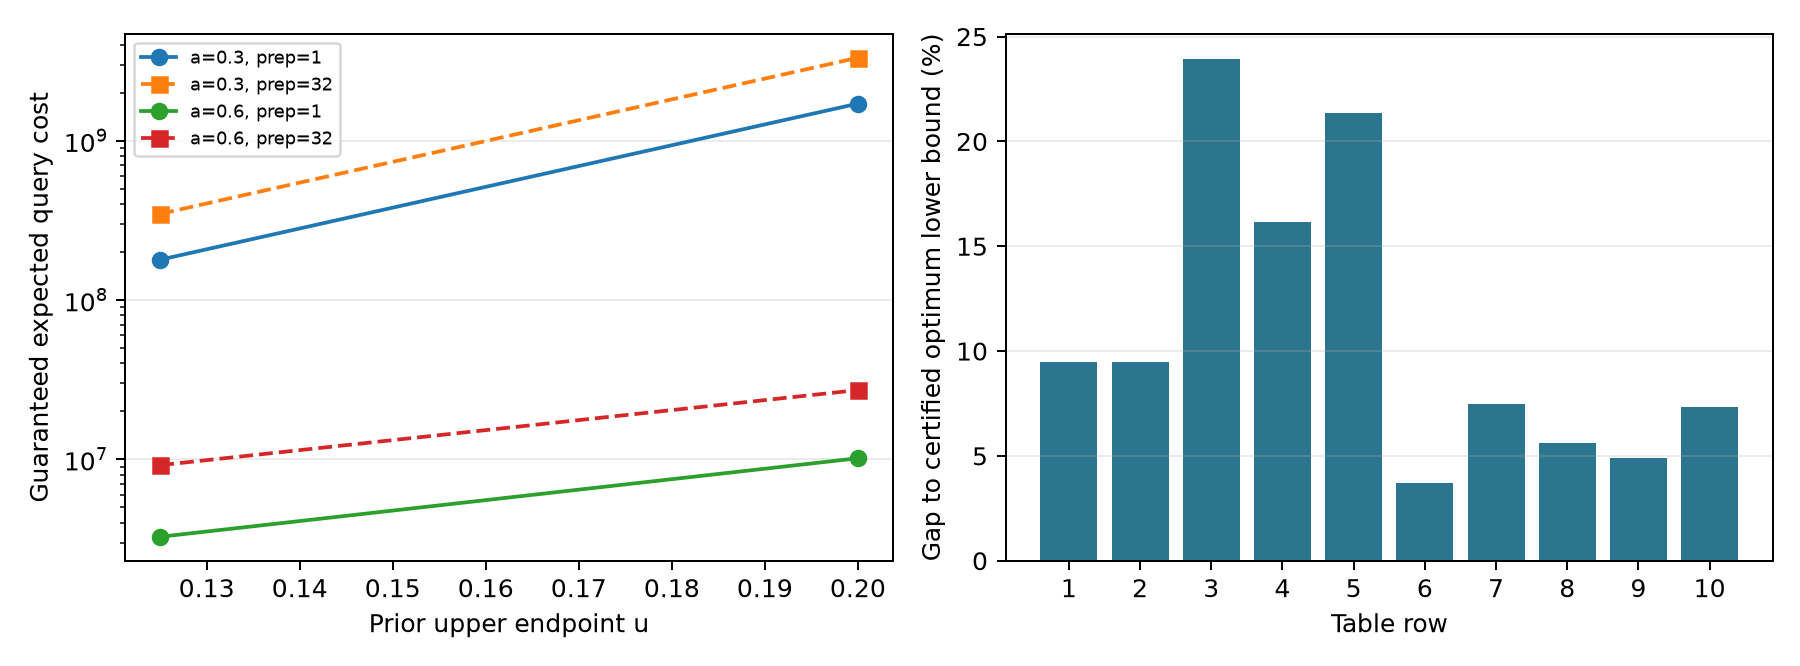
\includegraphics[width=\linewidth]{../../figures/selection_costs.png}
\caption{保証された期待query費用と事後的最適性Gap。
準備費用が違う条件は別の指定問題であり、各問題内では全候補の上限とoracle規約を揃える。}
\end{figure}

\paragraph{準備費用による切替}
$a=0.6,u=0.2,E=0.025,b=0.015$では、準備費用1で次数4、準備費用32で次数5を選ぶ。
受理コピー数は同一であり、後者の高い保証受理確率が、高価な準備の際に追加queryを
相殺する。理想多項式応答の厳密透過率区間から切替点を包囲でき、表示保証費用の交点は準備query単位で
約$12.34$となる。これは二つの固定多項式の比較であり、中間の全準備費用でこの二つだけが
最適候補になるとの主張ではない。

\begin{figure}[tb]
\centering
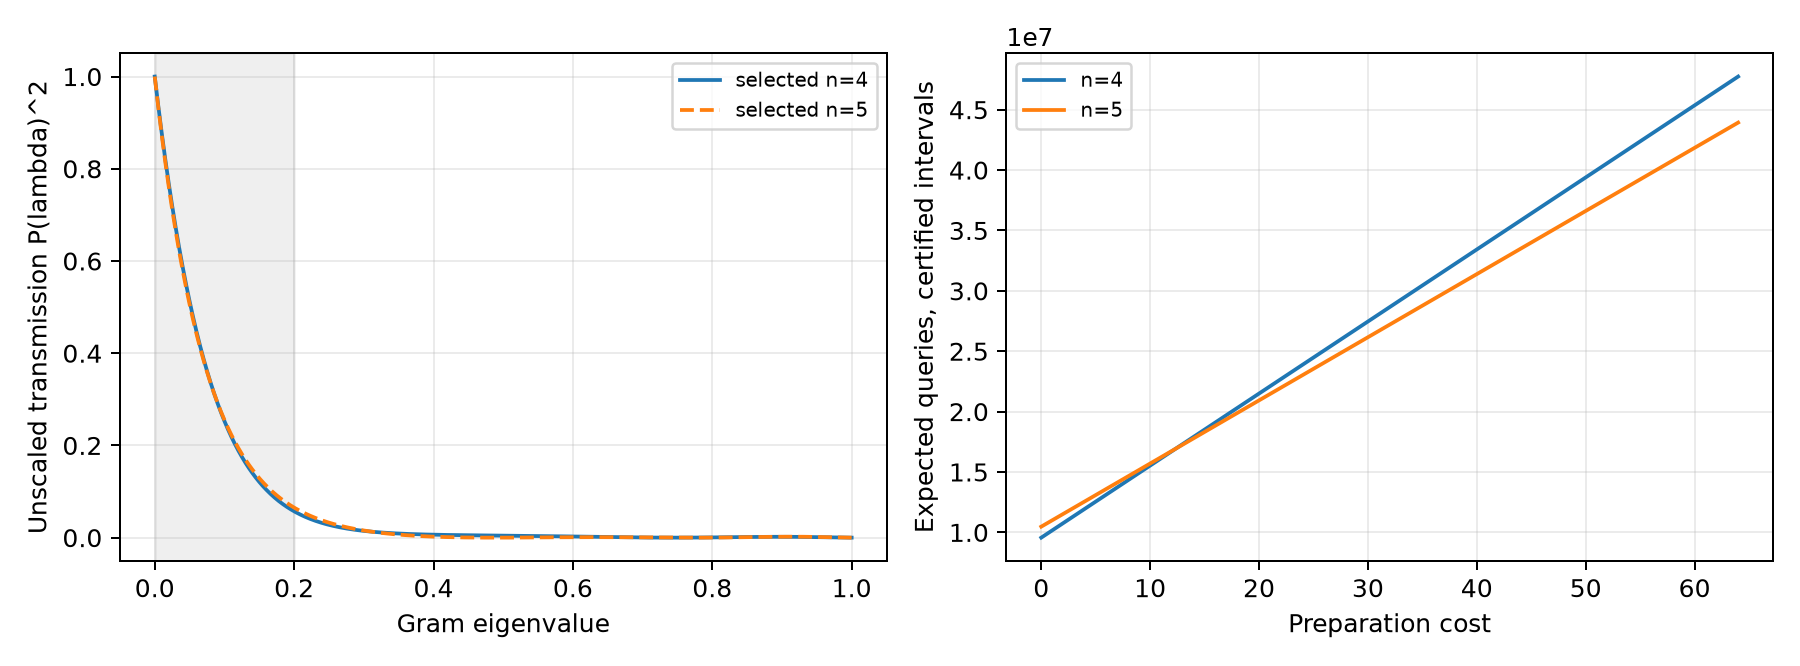
\includegraphics[width=\linewidth]{../../figures/selection_crossover.png}
\caption{同じ事前情報・バイアス配分に対する二応答。灰色は事前区間。
透過率包囲が費用の細い帯を与え、準備費用の増加で順序が変わる。}
\end{figure}

\paragraph{事前区間幅の費用}
命題\ref{prop:prior}の無制約上界を、証明済み多項式透過率が超えないことを確認した。
$a=0.3,E=0.025,c_\psi=1$では、$u=0.125$から$0.2$への拡大で、選択保証費用は
約$1.79\times10^8$から$1.71\times10^9$ queryへ増える。
大きい絶対費用は実用性の証拠ではなく、この頑健平均推定規約の限界を示す。

\begin{figure}[tb]
\centering
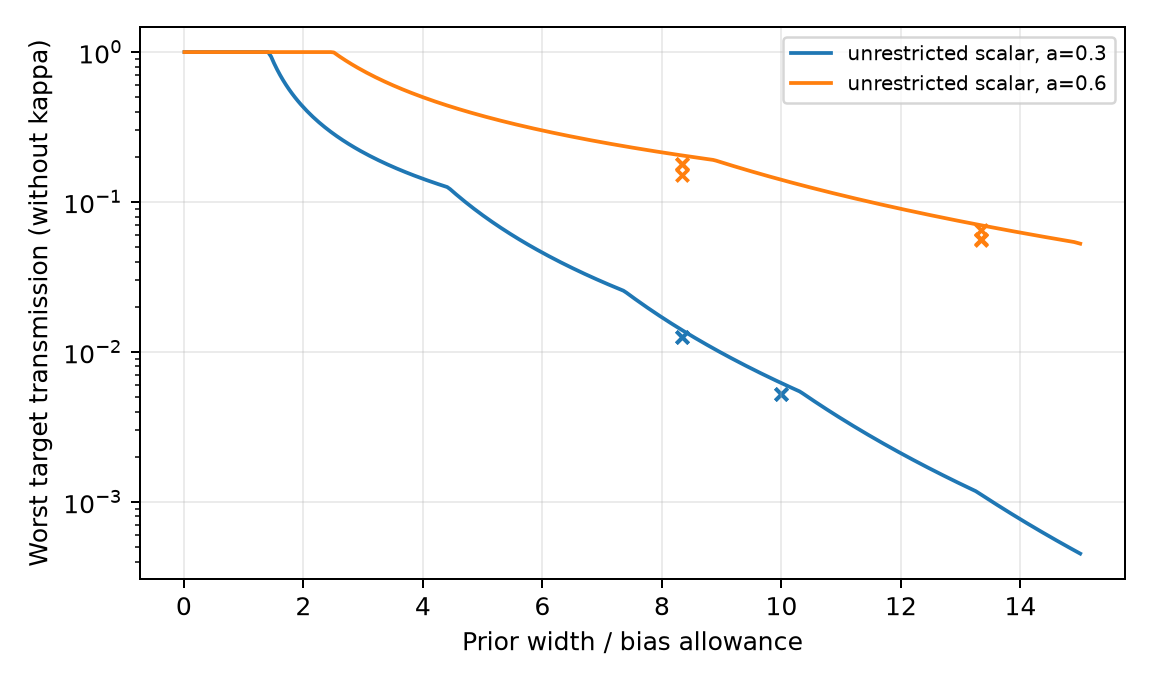
\includegraphics[width=.72\linewidth]{../../figures/selection_prior_limit.png}
\caption{事前区間幅／許容バイアスに対する無制約透過率上界と、証明済み多項式の値（×）。
両者から共通余裕$\kappa$を除いている。}
\end{figure}

\paragraph{位相・行列監査}
選択した全10多項式で位相合成に成功した。
保存位相から連続証明した最大振幅誤差は$3.63\times10^{-16}$で、全候補が予約バイアスを
満たす。実装成功下界への補正による費用増加率は$1+1.4\times10^{-14}$未満である。
これらは理想signal規約の結果であり、実機回転合成や雑音encodingへの保証ではない。

各選択に対し8次元正行列$B$を生成し、入力を固定計算基底$\ket0$とする。
生成側のHouseholder回転で重なりpromiseを制御するが、設計側には真の固有値も
その回転も与えない。各組の一例は最小値の$10^{-7}$上に励起値を置く。
16×16 signal行列へ全位相を適用し、32×32抽出ユニタリも明示的に構成した。
多項式目標との最大行列応答誤差は$5.55\times10^{-16}$、最大ユニタリ残差は
$6.33\times10^{-15}$であった。これはoracleの行列シミュレーションであり、物理ゲート合成ではない。

seed 20261027の独立なスカラー入力1,000例で、バイアスと受理確率の境界を確認した。
行列例ではseed 20261028のBernoulli・負の二項分布による集約標本計2,000反復を行い、
要求誤差に対するconfidence failureは零だった。
確率保証は定理から得るもので、有限観測で零だったことは整合確認にすぎない。
全係数・位相・入力行列・標本設定・厳密証明データを同梱する。

\section{理想回路・有限実行予算での精度}\label{sec:finite}
前節までの方式は成功サンプル数を固定し、期待費用を評価する。
ここでは回路・応答を理想的とし、ノイズを導入せず、全フィルタ試行を
$T\geq1$回で打ち切る。棄却時にも読出し1を予約して1試行を
$c_\psi+4n+1$単位と数えれば、総予算$B$から許される回数は
$T_n(B)=\lfloor B/(c_\psi+4n+1)\rfloor$である。
この保守的な計上を全候補に共通に課す。

実装成功重みを$w$、成功確率を$z=\sum_i p_iw(\lambda_i)$、
成功後の平均を$\mu=\sum_i p_i\lambda_iw(\lambda_i)/z$とする。
Gram実験では$w=\kappa^2P^2$。1試行の結果は、棄却・成功かつ0・成功かつ1の
3種類で、確率はそれぞれ$1-z,z(1-\mu),z\mu$である。よって
\[
 M\sim\operatorname{Bin}(T,z),\qquad
 K\mid M=m\sim\operatorname{Bin}(m,\mu).
\]
$M=0$なら値を返さず、$M>0$なら$\widehat e=K/M$を返す。
事前区間へのクリッピングはしない。値を返せない確率と、返せた場合の条件付き
二乗誤差を別々に示し、成功数を総実行数と混同しない。

\begin{proposition}[有限試行の厳密な法則]\label{prop:finite-law}
$q=1-z$、$C_T(z)=1-q^T$とし、
\[
 H_T(z)=\sum_{m=1}^T\binom Tm z^mq^{T-m}/m,\qquad h_T(z)=H_T(z)/C_T(z)
\]
とおく。このとき
\begin{equation}\label{eq:finite-mse}
 \Pr(M=0)=q^T,\qquad
 R_T=\mathbb E[(\widehat e-e)^2\mid M>0]
 = (\mu-e)^2+\mu(1-\mu)h_T(z).
\end{equation}
無出力も失敗と数えた許容誤差$E$での失敗確率は厳密に
\begin{equation}\label{eq:finite-failure}
 q^T+\sum_{m=1}^T\binom Tm z^mq^{T-m}
 \Pr\{\lvert\operatorname{Bin}(m,\mu)/m-e\rvert>E\}
\end{equation}
である。$h_T$は成功確率$z$に関して単調非増加で、
$h_T(1)=1/T$、$z\downarrow0$で$h_T(z)\to1$。
\end{proposition}
\begin{proof}
$M=m>0$で条件づけると、標本平均の平均は$\mu$、分散は
$\mu(1-\mu)/m$。二乗誤差と失敗事象をそれぞれ$M$で平均すれば両式が得られる。
正の二項分布は$\log(z/(1-z))$を自然母数とする指数型分布族なので、有限和を微分して
\[
 h_T'(z)=\frac{\operatorname{Cov}(1/M,M\mid M>0)}{z(1-z)}
 =\frac{1-h_T(z)\mathbb E[M\mid M>0]}{z(1-z)}\leq0.
\]
最後はJensen不等式による。端点の極限は有限和から従う。
\end{proof}

これらの逆二項モーメントと統計的事実は既知であり\cite{Znid,Drakakis}、
ショット雑音や$1/\sqrt T$則を新規性とはしない。
$M$を期待値$Tz$に置き換える近似は有限回では厳密でない。
$Tz$が小さい場合、値が返ったという条件下では成功数がほぼ1になるが、
同時に無出力が多くなる。$T$を増やすと分散項は減る一方、
固定フィルタのバイアス二乗は残る。MSEと固定信頼度の保証は異なる指標であり、
後者は式\eqref{eq:finite-failure}で評価する。

\begin{corollary}[固定締切での一様信頼度]\label{cor:deadline}
全入力で$z\geq s>0$、$0\leq\mu-e\leq b<E$なら、無出力も失敗と数えて
\begin{equation}\label{eq:deadline-confidence}
 \Pr\{\text{無出力 または }|\widehat e-e|>E\}
 \leq\min\{1,\,2[1-s(1-e^{-2(E-b)^2})]^T\}.
\end{equation}
よって信頼度$1-\delta$に十分な確定試行数は
\[
 T\geq\left\lceil\frac{\log(2/\delta)}
 {-\log[1-s(1-e^{-2(E-b)^2})]}\right\rceil.
\]
\end{corollary}
\begin{proof}
$M=m>0$なら$e$から$E$を超える偏差は$\mu$から少なくとも$E-b$の偏差を必要とし、
Hoeffding上界は$2e^{-2m(E-b)^2}$。$m=0$でも右辺は2なので失敗の上界となる。
二項分布の母関数で平均し、$z\geq s$を使えば従う。
\end{proof}
これは既知の集中不等式と母関数の帰結であり、新しい集中不等式とはしない。
バイアス・成功確率の証明書を、期待費用だけでなく固定締切での信頼度に接続する。

\begin{theorem}[条件付きリスクの3固有値への縮約]\label{thm:three}
$T,a,u$を固定し、連続な重み$0\leq w\leq1$が$[0,u]$上で正とする。
許される全ての有限スペクトル・初期重みについての式\eqref{eq:finite-mse}の最大値は
\begin{equation}\label{eq:three}
 a\delta_e+(1-a)\{\theta\delta_x+(1-\theta)\delta_y\},\qquad
 0\leq e\leq u,\quad e\leq x,y\leq1,\quad0\leq\theta\leq1
\end{equation}
で達成される。固有値の重複を許すので、目標質量は$a$を超えてもよい。
\end{theorem}
\begin{proof}
任意の入力から$e$での質量$a$を確保し、残りを元の有限支持上の確率測度$r$とする。
必要なら$r$にも$e$を含める。この入力の事後平均$\mu$を固定し、
\begin{equation}\label{eq:moment-lp}
 \int dr=1,\qquad
 \int(x-\mu)w(x)\,dr(x)=\frac{a}{1-a}(\mu-e)w(e),\qquad r\geq0
\end{equation}
の下で$\int w\,dr$を最小化する。元の測度が実行可能である。
等式制約は高々2本なので、有限LPの最適基本解は高々2つの正の重みで表せる。
新しい入力は$\mu$を保ち$z$を減らすため、$h_T$の単調性から条件付きMSEは減らない。
目標の1点を加えて高々3固有値になる。逆に式\eqref{eq:three}は許される入力である。
そのパラメータ集合はコンパクトで、$z\geq a\min_{[0,u]}w>0$よりリスクは連続。
したがって最大値を達成する。
\end{proof}

これは既知のモーメント集合・基本解の議論\cite{Winkler,Pinelis}を、このリスクへ適用した
正確な低次元化である。バイアス・分散・成功確率の別々の最悪例が同時に成立すると
仮定するものではない。常に3点が必要とは主張しない。また格子性を持つ失敗確率、
クリッピングした推定量、別の停止則に同じ縮約が成り立つとは述べない。

\paragraph{計算可能な一様上界と選択.}
全入力で$z\geq s>0$、$0\leq\mu-e\leq b$なら、
$t_b=\min\{u+b,1/2\}$、$v_b=t_b(1-t_b)$に対し
\begin{equation}\label{eq:finite-upper}
 R_T\leq b^2+v_bh_T(s),\qquad \Pr(M=0)\leq(1-s)^T.
\end{equation}
上端零化の場合、無出力の上界は最小目標透過率と上端の2点で達成する。
MSE上界は各最悪量が両立しない場合があり、一般に等号とはしない。
\[
 A_T=\frac{1-(1-s)^{T+1}}{(T+1)s},\quad
 B_T=\frac{1-[1+(T+1)s](1-s)^{T+1}}{(T+1)(T+2)s^2}
\]
とおくと、厳密な計算用上界は
\begin{equation}\label{eq:inverse-upper}
 h_T(s)\leq\min\left\{1,
 \frac{A_T+3B_T-\frac52(1-s)^T}{1-(1-s)^T}\right\}.
\end{equation}
実際、$m\geq1$で$1/m\leq1/(m+1)+3/[(m+1)(m+2)]$。
右辺2項の全二項分布での期待値が$A_T,B_T$であり、$m=0$分を除くと
$5(1-s)^T/2$を差し引く。実装では有理入力と外向き180bit累乗で包絡する。
数値積分は厳密法則の照合用に限り、選択の証明書には用いない。

有限候補群について$T_n(B)$でこのMSE上界を最小化し、
無出力確率の保証上界を0.05以下に制限する。
量子計算をしない事前中点も、最悪MSE$u^2/4$・無出力0の候補として含める。
最適性は候補群の計算した上界に対してのみであり、一般的な量子推定の最適性ではない。
ポストセレクションの既存議論\cite{Combes}と同様、棄却された実行を除外した
条件付き精度だけから優位性を結論しない。

\section{物理模型への適用と有限サンプリング実験}\label{sec:physical}
開放端横磁場イジング模型
$H=-\sum_{i=1}^NX_i-J\sum_{i=1}^{N-1}Z_iZ_{i+1}$と初期状態
$\ket+^{\otimes N}$を用いる。この模型での量子フィルタ評価は既存であり\cite{QETU}、
応用名を新規性とはしない。$N=4,6,8$、$v=(N-1)J=0.4,0.8$の6条件。
サイズとともに$J$も変わるので、熱力学的なスケーリング実験ではない。

\paragraph{対角化前に与える解析的な事前情報.}
$\Delta=2-v$、$t^2=v^2/(N-1)$、$d=t^2/\Delta$とする。
非相互作用の積状態のエネルギーは$-N$、直交ブロックは
$QHQ\succeq(-N+\Delta)Q$であり、異なる結合がX基底で異なる2スピンを反転するので
$\|QV\ket+^{\otimes N}\|^2=t^2$。基底状態を$c\ket+^{\otimes N}+q$と分けると、
変分上界$E_0\leq-N$とブロックの固有方程式から
\[
 q=-(QHQ-E_0)^{-1}QV\ket+^{\otimes N}c,\quad
 -N-E_0\leq t^2/\Delta,\quad \|q\|\leq(t/\Delta)|c|.
\]
よって$L=-N-d\leq E_0\leq U=-N$、重なり下界は
$a=1/(1+t^2/\Delta^2)$。
$R=N+v$、$G=(H-LI)/(R-L)$、$u=d/(R-L)$、$E=u/8$とする。
物理エネルギーの精度は$d/8$で、事前中点の保証誤差$d/2$より4倍厳しい。
真の固有値・重みは選択を固定した後の監査にだけ用いる。
事前境界の導出は非相互作用模型のギャップを使う。この弱結合実験で
gap-free方式の優位性を確認したとはしない。

\paragraph{Hamiltonianへの実装上の写像.}
エネルギー平均にスカラー定理を適用するため、$Y=2G-I$の理想的な正規化
Hermitian信号を仮定する。$P(x)=\sum c_kT_k(2x-1)$なら
$F(y)=P((y+1)/2)$を偶・奇部分に分け、各々をQSP合成できる。
$|F|\leq1$より各部分も$[-1,1]$で有界。安全係数0.95で合成し、
Hermitian抽出とLCU平均を使うと振幅は$0.475P(G)$となる。
追加の1/2を非自明なフィルタ候補に計上する。無フィルタ基準は抽出を省き成功確率1。
直列呼出しは高々$4n$、
準備費用は感度パラメータ$c_\psi=N$とした。実ゲート深さではない。
$Y$をPauli LCUで作る係数ノルムは$(2R+|R+L|)/(R-L)$で一般に1を超え、
正規化信号へ変換する追加操作の費用は含めない。したがって理想oracleの比較である。
$Y$の制御encodingへのHadamard testを1回行えば、結果確率は
$(1+\langle Y\rangle)/2=\langle G\rangle$となる。平方根Hamiltonianを無料で
仮定せずに、Bernoulli型energy読出しを実現する。

4スピン・$v=0.8$では積状態のバイアス0.053411が目標0.022222を超えたが、
元の次数7応答で0.000368となった。元の6応用条件すべてでバイアス目標を達成。
試したChebyshev型の保証費用は選択応答の1.001--1.173倍、認証されたpower型の
3条件では5.03--19.02倍。他の3条件は次数上限内の試した候補に認証がない。
全チューニングに対する優位性ではなく、絶対費用も大きい。
元の応用位相の連続誤差上界は最大$2.04\times10^{-16}$だが、以下では本人指定の
理想回路条件に従い目標多項式そのものを厳密とし、測定の有限性だけを加える。

\paragraph{有限予算での選択と再現.}
元の認証済み候補に、$b/u\in\{1/32,1/16,1/8,1/4,1/2\}$、
$n\in\{1,2,3,4,5,6,8,10,12,16\}$のLP候補を加える。
設計は$0.98b$、連続証明は$0.99b$で、認証に失敗した候補は除く。
無フィルタ平均も加えた6候補群の大きさは27,27,24,20,19,15。
事前中点は別の候補とする。総予算$B=10^2,10^3,\ldots,10^9$ごとに
式\eqref{eq:finite-upper}--\eqref{eq:inverse-upper}の上界を最小化し、
無出力上界を0.05以下に制限する。48条件のうち21条件では事前中点が選ばれた。
予算増加に伴い次数と誤差配分が変わる。選択には対角化の真値を使わない。

\begin{figure}[tb]
\centering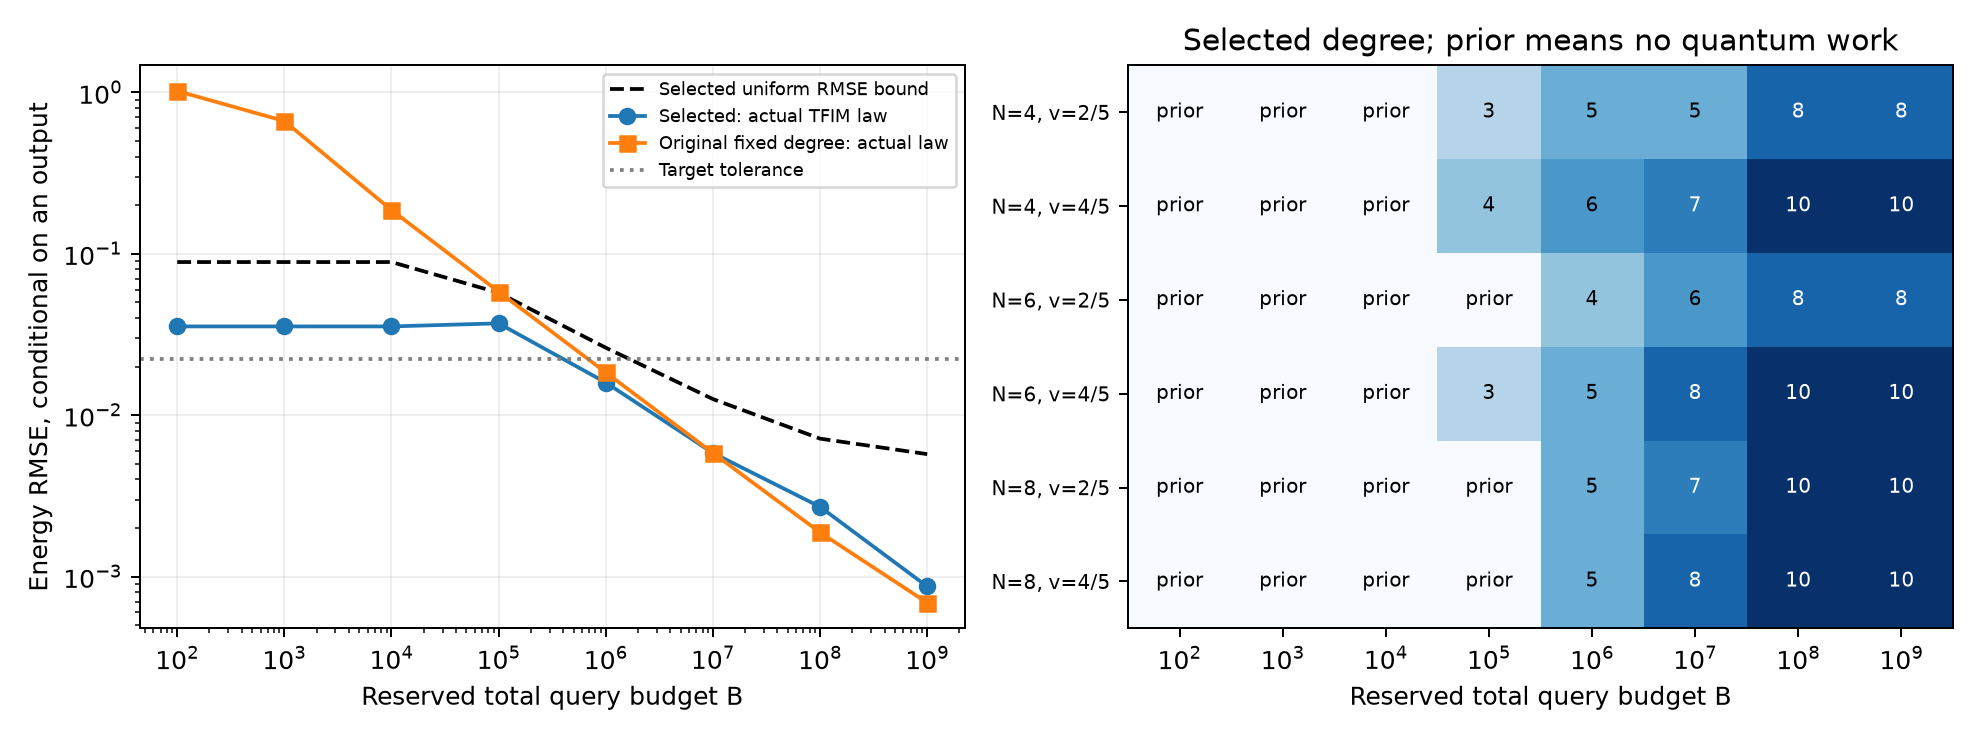
\includegraphics[width=\linewidth]{../../figures/finite_budget.png}
\caption{有限予算選択。左の黒線は一様RMSE上界、色線は4スピン・$v=0.8$での
厳密法則の数値評価。右は6事前条件で選ばれた次数。priorは量子計算なし。
一様上界の改善は各個別入力での実際のリスク改善を意味しない。}
\end{figure}

3固有値縮約は、21固有値を持つ100個の独立な入力でも検査した。
モーメントLP後は全例で支持が高々3点、平均を維持し、受理確率は増えず、
条件付きMSEも減らなかった。観測されたリスク増加は最大3.95倍。
これは証明した縮約の数値照合であり、連続最悪ケースを数値的に認証したものではない。

\paragraph{有限回の精度、信頼度、バイアスの下限.}
4スピン・$v=0.8$で元の次数7応答を固定した結果は次の通り。
\begin{center}\small
\begin{tabular}{rrrr}
\toprule
$B$ & 条件付きenergy RMSE & 無出力 & 精度違反確率\\
\midrule
$10^2$ & $1.021$ & $0.711$ & $1.000$\\
$10^6$ & $0.01840$ & $<10^{-12}$ & $0.2265$\\
$10^7$ & $0.005830$ & $<10^{-12}$ & $0.000157$\\
\bottomrule
\end{tabular}
\end{center}
$B=10^6$ではRMSEが目標0.022222より小さくても、精度違反は約22.65\%ある。
したがってRMSEだけから95\%信頼度を述べられない。
確率は式\eqref{eq:finite-failure}の二項混合を数値評価し、省略する成功数の確率は
約$10^{-12}$以下とした。正規近似ではないが、厳密有理区間証明とも区別する。

3応答を固定して$T=10^0,\ldots,10^{12}$を変えると、標本誤差の減少から
バイアスで頭打ちになる領域へ移る。次数4,7,10の物理energyバイアスはそれぞれ
0.000763、0.000368、0.000157であり、ショット数だけを増やしても消せない。
合計114バッチで各20,000回、計2,280,000回の独立集約二項サンプリングを行った。
実測MSEは厳密法則の数値値と整合し、最大の差はMonte Carlo標準誤差の3.31倍。
予算実験でランダム成功数を期待値で置き換えた予測とのMSE比は0.280--1.293だった。
別に厳密有理和・包絡演算の183チェックを通した。

\begin{figure}[tb]
\centering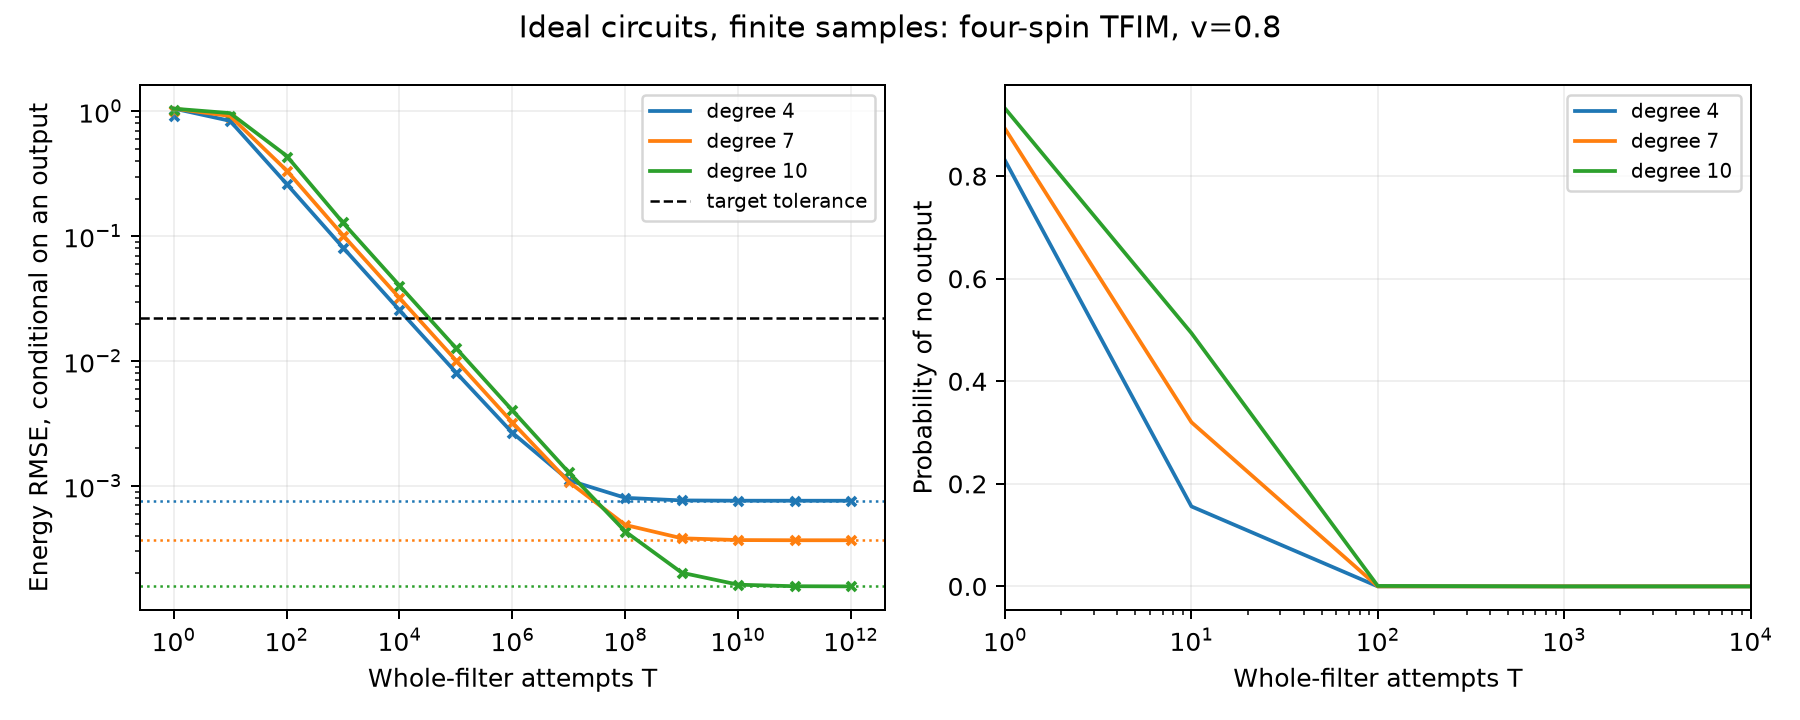
\includegraphics[width=\linewidth]{../../figures/finite_precision.png}
\caption{理想回路・有限サンプリング。線は条件付きRMSEの法則、十字はMonte Carlo、
点線はバイアス下限。右は無出力確率。目標線は許容誤差で、信頼区間の境界ではない。}
\end{figure}

頑健選択は保守的である。同じ代表例の$B=10^8$では次数10を選び、実際のRMSEは
0.00270で、元の次数7の0.00188より大きい。最小化したのは候補群内の一様保証上界で、
個別スペクトルの実リスクではない。小規模・古典的に解ける鎖なので、量子優位、
熱力学的スケーリング、QET-U等への優位性を示さない。追加の成果は、有限予算の
精度と無出力を明記した目的、スペクトル縮約、再現可能な理想サンプリング検証である。


\section{考察と限界}
本選択則は、与えられた事前情報のもとで、どの実多項式・次数・有限誤差配分が
最悪再試行費用の保証を小さくするかに答える。
上端零化の比較により、目的関数が正確な操作的意味を持つクラスへ制限する費用を
明示できる。連続可行性と双対証明は、少数の既存関数に対する改善と、
制限した最適値への近さを区別する。

推定器と再試行規約の制限は大きい。振幅増幅、coherent recycling、仮想フィルタ、
位相推定型の読出し、適応的な事前情報取得は資源依存性を変え得る。
QET-Uや他の基底energy推定器は別の情報・読出し条件を扱い\cite{QETU,Accurate}、
本結果はそれらの下界ではない。重なり下界の取得費、物理ゲート深さ、誤り訂正、
化学系encoding、実機雑音は評価していない。連続な誤差配分全体での最適性も、
有限配分格子からは主張しない。

最悪条件は個別スペクトルには保守的であり、事前区間幅に比べ許容バイアスが小さいと
絶対費用は大きくなる。これは関数の柔軟性だけでは弱い事前情報の費用を消せないことを
示す。本稿は最適QSVT関数族の発明や一般量子優位を主張せず、
構造的帰着と指定された頑健選択問題への再現可能な証明付き回答を示す。

\section{結論}
全再試行・読出しqueryを算入した、事前情報だけによるgap-free平均推定のフィルタ選択を
定式化した。制御された上端零化は、一般の実応答を最悪受理確率が正確に分かるクラスへ
結びつける。その結果、費用上下界を伴う凸多項式設計と、選択後の連続位相検証が可能に
なる。状態準備費用や事前情報によって応答を変えるべき場合を示す一方で、
固定フィルタ平均推定器が依然として高価になる領域も明確にした。

有限試行の拡張では無出力、条件付きMSE、信頼度を分離した。
3固有値縮約は、別々の最悪量を同時達成できると仮定せずに最悪リスクを特徴づける。
数値選択は有限候補群の認証上界の最小化であり、各入力の実際の誤差改善を保証しない。
理想回路でも有限サンプリングと固定応答のバイアスは残る。

\appendix
\section{厳密演算と連続証明}
$p(x)=\sum_{j=0}^na_jx^j$を$[0,L]$で表すBernstein係数は
\[
 b_i=\sum_{j=0}^i a_jL^j\frac{\binom ij}{\binom nj}
\]
である。基底が非負で和が1なので、値は係数の最小・最大の間にある。
de Casteljau中点分割の各下端を下向き、上端を上向きに$2^{-220}$単位の整数へ丸め、
包囲の包含を分割ごとの帰納法で維持する。保存十進係数・位相は厳密有理数であり、
浮動小数最適化の出力そのものを厳密証明とはしない。

結合残差には$w=P^2\geq0$と$A_b=ab/(1-a)$を用いる。
$e\in[e_0,e_1]$、$x\in[x_0,x_1]$のboxで
\[
 (x-e-b)w(x)-A_bw(e)\leq(x-e_0-b)w(x)-A_bw(e)
\]
とし、$xw(x)$と$w(x)$を同じ次数のBernstein基底で包囲して差を取る。
$A_bw(e)$の下界を引いた値が非正ならbox全体で成立する。
$x_1\leq e_0+b$なら追加検査不要である。
node数・深さ上限で解けなければ未証明として棄却し、格子の成功で置き換えない。
この手順の全候補に対する終了・最適化収束は主張しない。

位相検証ではQSPの上段を$(P(s),i\sqrt{1-s^2}Q(s))$と書くと、1stepの漸化式は
\[
 P_{\rm new}=e^{i\phi}[sP-(1-s^2)Q],\qquad
 Q_{\rm new}=e^{-i\phi}[P+sQ]
\]
となる。偶signal次数では対角応答が偶多項式なので、虚部を$s^2$の多項式として扱える。
各sin/cosを有理Taylor余剰で包み、複素区間演算後の誤差多項式を同じBernstein法で評価する。
したがって位相誤差境界は連続区間を覆い、別途行う行列格子検査だけに依存しない。

$\delta=.05$の標本数には$\log40=\log5+3\log2$の有理上界を使う。
\[
 \log x=2\sum_{j=0}^{m-1}\frac{z^{2j+1}}{2j+1}+R_m,\quad
 z=\frac{x-1}{x+1},\quad
 0\leq R_m\leq\frac{2z^{2m+1}}{(2m+1)(1-z^2)}
\]
を用いて有理数の要求標本数を上向きに整数化し、未検査の浮動小数ceilingに頼らない。

\section{形式検証の範囲}
\texttt{lean/Selection.lean}はLean 4.35.0 / Mathlib v4.35.0で
\texttt{lake build Selection}に成功し、
\texttt{lake env lean SelectionAudit.lean}にも成功した。
検証対象の5補題は、二点分母払いの同値性、目標質量がちょうど$a$の有限混合への十分性、
順序付き減衰係数による二点条件の保存、二つの入力境界からの上端受理係数の代数、
およびstationarity補正付きweak dualityである。
使用公理は\texttt{propext}、\texttt{Classical.choice}、\texttt{Quot.sound}のみで、
該当証明に\texttt{sorry}、\texttt{admit}、独自axiom、\texttt{native\_decide}はない。

実際の質量$p_0\geq a$への拡張、関数空間・最適化の議論、事前区間幅の包絡、
Bernsteinアルゴリズム、位相区間証明、行列還元、query実装、集中不等式は、
手証明または計算証明であり、全体をLean形式化したものではない。
同じtarget用のworkflowは用意したが、遠隔CI成功は主張せず、今回報告する成功はローカルである。
補足記録にソースhashと実行ログを含める。

\section{再現性と計算の範囲}
同梱する実行入口は以下である。
\begin{itemize}
\item \texttt{filter\_selection.py}：設計と連続証明。
\item \texttt{selection\_qsp.py}：位相合成と応答包囲。
\item \texttt{selection\_matrix\_audit.py}：全block行列監査。
\item \texttt{selection\_figures.py}：表・図・summary生成。
\item \texttt{check\_selection\_certificates.py}：厳密算術の対照検査。
\end{itemize}
共有算術moduleは\texttt{selection\_certificates.py}である。
設計JSONはソースhash、取得可能なら基準Git版、厳密係数・dual境界、証明診断、
パラメータ、依存版を記録する。位相JSONは入力設計のhash、行列JSONは設計と位相の
hashを記録する。厳密費用の有理数と表示用近似値を併記し、ソースmanifestも含める。

本実験は小さな人工prior格子に限定される。既存族のパラメータ探索も有限であり、
各族の任意調整に対する最適値と比較したものではない。
証明付き候補が返らない族について架空の性能値を報告しない。
全本実験は$u>4E$を満たす。
この非自明性を満たさなかった初期診断条件は本実験から除外し、研究記録に棄却した
評価設計として残した。

今回の確認用原稿では本人の指定により著者情報を省略する。
候補導出、執筆、実装にはAI支援を使用しており、生成と検証を同一視せず、
実際の検査範囲を上記のとおり明示する。
preprint serverへのupload・投稿は行っていない。

\begin{thebibliography}{99}
\bibitem{Gilyen} A. Gily\'en, Y. Su, G. H. Low, and N. Wiebe, ``Quantum singular value transformation and beyond: exponential improvements for quantum matrix arithmetics,'' STOC (2019), pp. 193--204, doi:10.1145/3313276.3316366; arXiv:1806.01838.
\bibitem{Martyn} J. M. Martyn, Z. M. Rossi, A. K. Tan, and I. L. Chuang, ``Grand Unification of Quantum Algorithms,'' \emph{PRX Quantum} \textbf{2}, 040203 (2021), doi:10.1103/PRXQuantum.2.040203.
\bibitem{Ge} Y. Ge, J. Tura, and J. I. Cirac, ``Faster ground state preparation and high-precision ground energy estimation with fewer qubits,'' \emph{J. Math. Phys.} \textbf{60}, 022202 (2019), doi:10.1063/1.5027484; arXiv:1712.03193.
\bibitem{LinTong} L. Lin and Y. Tong, ``Optimal polynomial based quantum eigenstate filtering with application to solving quantum linear systems,'' \emph{Quantum} \textbf{4}, 361 (2020), doi:10.22331/q-2020-11-11-361.
\bibitem{Lu} S. Lu, M. C. Ba\~nuls, and J. I. Cirac, ``Algorithms for Quantum Simulation at Finite Energies,'' \emph{PRX Quantum} \textbf{2}, 020321 (2021), doi:10.1103/PRXQuantum.2.020321.
\bibitem{He} M.-Q. He, D.-B. Zhang, and Z. D. Wang, ``Quantum Gaussian filter for exploring ground-state properties,'' \emph{Phys. Rev. A} \textbf{106}, 032420 (2022), doi:10.1103/PhysRevA.106.032420.
\bibitem{FQPE} G. Lee, M. Kang, J. Hong, S. Fomichev, and J. Huh, ``Filtered Quantum Phase Estimation,'' arXiv:2510.04294v2 (2026).
\bibitem{Wall} M.-A. Filip and N. Fitzpatrick, ``Beyond asymptotic reasoning: the practicalities of a quantum ground state projector based on the wall-Chebyshev expansion,'' arXiv:2508.00533v3 (2026), doi:10.1088/2058-9565/ae2887.
\bibitem{Constrained} Y. Dong, J. B. Larsen, L. Lin, and R. Sarkar, ``Constrained minimax approximation for quantum signal processing,'' arXiv:2608.30937 (2026).
\bibitem{Charnes} A. Charnes and W. W. Cooper, ``Programming with linear fractional functionals,'' \emph{Naval Research Logistics Quarterly} \textbf{9}, 181--186 (1962), doi:10.1002/nav.3800090303.
\bibitem{Farouki} R. T. Farouki, ``The Bernstein polynomial basis: A centennial retrospective,'' \emph{Computer Aided Geometric Design} \textbf{29}, 379--419 (2012), doi:10.1016/j.cagd.2012.03.001.
\bibitem{DongPhase} Y. Dong, X. Meng, K. B. Whaley, and L. Lin, ``Efficient phase-factor evaluation in quantum signal processing,'' \emph{Phys. Rev. A} \textbf{103}, 042419 (2021), doi:10.1103/PhysRevA.103.042419.
\bibitem{Symmetric} Y. Dong, L. Lin, H. Ni, and J. Wang, ``Robust iterative method for symmetric quantum signal processing in all parameter regimes,'' \emph{SIAM J. Sci. Comput.} \textbf{46}, A2951--A2971 (2024); arXiv:2307.12468.
\bibitem{QETU} Y. Dong, L. Lin, and Y. Tong, ``Ground state preparation and energy estimation on early fault-tolerant quantum computers via quantum eigenvalue transformation of unitary matrices,'' \emph{PRX Quantum} \textbf{3}, 040305 (2022), doi:10.1103/PRXQuantum.3.040305.
\bibitem{Accurate} A. Dutkiewicz, T. E. O'Brien, and S. Polla, ``Accurate ground state energy estimation with noise and imperfect state preparation,'' arXiv:2603.21873v2 (2026).
\end{thebibliography}

\end{document}
